\[
=8.15<\chi_{(4-2-1)\times 2}^{2}(0.01)=9.21
\]

故在显著性水平 $\alpha=0.01$ 下我们不能拒绝二次多项式拟合的合适性. 但由于 $p$ 值小于 $0.05$, 有迹象表明二次多项式拟合不是非常好.

利用轮廓分析方法, 我们不用对二次多项式损失施加限制, 就能检验主尺骨中钙量损失的轮廓的平行性和相合性. \hfill$\blacksquare$

对于比单因子 MANOVA 更一般的实验设计, 波托夫与罗伊的生长曲线模型也适用. 但此时 $\hat{\boldsymbol{\beta}}$ 不再由\hyperref[eq:6-78]{式(6-78)}给出, 而且其协方差矩阵的表达式远比\hyperref[eq:6-79]{式(6-79)}复杂. 至于更多的例子和进一步的检验, 建议读者参阅(见文献[14]).

对我们所考虑的模型还有许多改进方法, 其中包括:

(a) 解除对多项式生长的限制. 采用非线性参数模型或者甚至采用非参数样条分析.

(b) 限定协方差阵取某种特殊形式, 使得对相同的个体有等相关的响应.

(c) 对相同的个体, 在某一时段观测一个以上的响应变量, 这就导致生长曲线模型的多元形式.

\section{对分析多元模型的展望和建议}
\phantomsection\label{sec:6.10}

我们强调指出, 对多个指标特征, 控制作出任何错误决策的总概率是很重要的. 正如本章中的那些例子所指明的那样, 在检验两种或两种以上处理的相等性时, 这点尤为重要. 对具有单一 $p$ 值的检验问题, 作一个多元检验要比完成大量一元检验更可取. 这一结果告诉我们: 通过变量分析和分批进行的办法去接近某一个变量究竟是否值得.

我们建议采用一个多元检验, 而非 $p$ 个一元检验, 因为下一个例子将说明, 一元检验忽略了一些重要的信息, 因而可能给出误导的结论.

\noindent\textbf{例 6.16}\quad (对均值差比较多元检验与一元检验)

假定从两个组分别随机选取 10 个实验单元, 并收集两个变量 $X_1$ 与 $X_2$ 的测量值. 下面列出这两个变量的假想数据, 这些数据的散布图和边际点图如\hyperref[fig:6.6]{图 6.6} 所示.

\begin{center}
\begin{tabular}{ccc}
$x_1$&$x_2$&组别\\ \midrule
5.0&3.0&1\\
4.5&3.2&1\\
6.0&3.5&1\\
6.0&4.6&1\\
6.2&5.6&1\\
6.9&5.2&1\\
6.8&6.0&1\\
5.3&5.5&1\\
6.6&7.3&1\\
7.3&6.5&1\\
4.6&4.9&2\\
4.9&5.9&2\\
4.0&4.1&2\\
3.8&5.4&2\\
6.2&6.1&2\\
5.0&7.0&2\\
5.3&4.7&2\\
7.1&6.6&2\\
5.8&7.8&2\\
6.8&8.0&2\\
\end{tabular}
\end{center}

\begin{mvfigure}
\centering
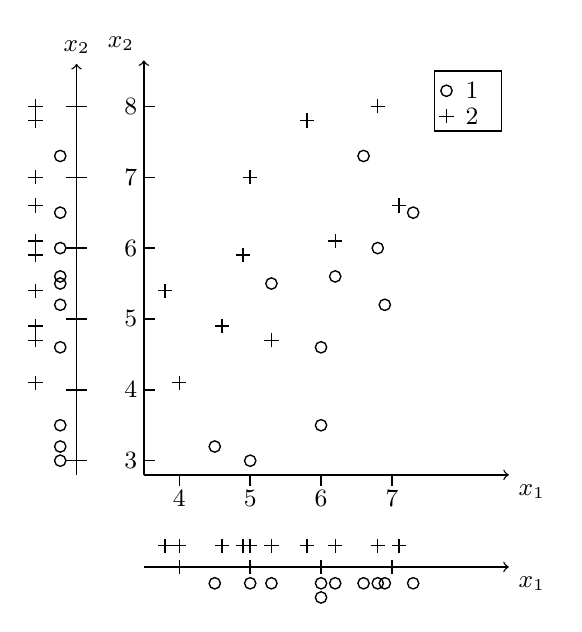
\begin{tikzpicture}[scale=0.9,line width=0.5pt]
% ===== 主散布图 =====
\draw[->] (3.5,2.8)--(8.65,2.8) node[below right,font=\small]{$x_1$};
\draw[->] (3.5,2.8)--(3.5,8.65) node[above left,font=\small]{$x_2$};
\foreach \t in {4,5,6,7}{\draw (\t,2.8)--(\t,2.64); \node[below,font=\small,fill=white,inner sep=0.6pt] at (\t,2.62){$\t$};}
\foreach \t in {3,4,5,6,7,8}{\draw (3.5,\t)--(3.66,\t); \node[left,font=\small,fill=white,inner sep=0.6pt] at (3.44,\t){$\t$};}
% 第1组（圆圈）
\foreach \x/\y in {5.0/3.0,4.5/3.2,6.0/3.5,6.0/4.6,6.2/5.6,6.9/5.2,6.8/6.0,5.3/5.5,6.6/7.3,7.3/6.5}{\draw (\x,\y) circle (0.08);}
% 第2组（加号）
\foreach \x/\y in {4.6/4.9,4.9/5.9,4.0/4.1,3.8/5.4,6.2/6.1,5.0/7.0,5.3/4.7,7.1/6.6,5.8/7.8,6.8/8.0}{\draw (\x-0.1,\y)--(\x+0.1,\y); \draw (\x,\y-0.1)--(\x,\y+0.1);}
% 图例
\draw (7.6,7.65) rectangle (8.55,8.5);
\draw (7.77,8.22) circle (0.08); \node[right,font=\small] at (7.9,8.22){1};
\draw (7.67,7.86)--(7.87,7.86); \draw (7.77,7.76)--(7.77,7.96); \node[right,font=\small] at (7.9,7.86){2};
% ===== 左侧边际点图 =====
\draw[->] (2.55,2.8)--(2.55,8.6) node[above,font=\small]{$x_2$};
\foreach \t in {3,4,5,6,7,8}{\draw (2.4,\t)--(2.7,\t);}
\foreach \y in {4.1,4.7,4.9,5.4,5.9,6.1,6.6,7.0,7.8,8.0}{\draw (1.97,\y-0.1)--(1.97,\y+0.1); \draw (1.87,\y)--(2.07,\y);}
\foreach \y in {3.0,3.2,3.5,4.6,5.2,5.5,5.6,6.0,6.5,7.3}{\draw (2.32,\y) circle (0.08);}
% ===== 底部边际点图 =====
\draw[->] (3.5,1.50)--(8.65,1.50) node[below right,font=\small]{$x_1$};
\foreach \t in {4,5,6,7}{\draw (\t,1.40)--(\t,1.60);}
\foreach \x in {3.8,4.0,4.6,4.9,5.0,5.3,5.8,6.2,6.8,7.1}{\draw (\x-0.1,1.80)--(\x+0.1,1.80); \draw (\x,1.70)--(\x,1.90);}
\foreach \x/\y in {4.5/1.27,5.0/1.27,5.3/1.27,6.0/1.27,6.0/1.07,6.2/1.27,6.6/1.27,6.8/1.27,6.9/1.27,7.3/1.27}{\draw (\x,\y) circle (0.08);}
\end{tikzpicture}
\phantomsection\label{fig:6.6}\mvcap{图 6.6\quad 两组数据的散布图和边际点图}
\end{mvfigure}
